%----------------------------------------------------------------------------------------
%    PACKAGES AND THEMES
%----------------------------------------------------------------------------------------

\documentclass[aspectratio=169,xcolor=dvipsnames]{beamer}
\setbeameroption{show notes} %TODO: Thomas a enlever avant la presentation
\usetheme{SimplePlus}

\useoutertheme{miniframes}  % Adds horizontal navigation dots at the top for subsections

\usecolortheme{} 

\setbeamercolor{block title}{bg=structure,fg=white}  % Navy blue background for block titles
\setbeamercolor{block body}{bg=structure!10,fg=black}  % Light navy tint for block body

\definecolor{darkwine}{RGB}{128,0,32}  % Dark red wine
\newenvironment{errorblock}[1]{%
\begingroup%
\setbeamercolor{block title}{bg=darkwine,fg=white}%
\setbeamercolor{block body}{bg=structure!05,fg=black}%  % Very close to white background
\begin{block}{#1}%
}{\end{block}\endgroup}

\usepackage{comment}
\usepackage{hyperref}
\usepackage{graphicx} % Allows including images
\usepackage{booktabs} % Allows the use of \toprule, \midrule and \bottomrule in tables
\usepackage{array} % Allows >{\centering\arraybackslash} in tabular

% Define hyphenation command
\newcommand{\hyp}{-}

%----------------------------------------------------------------------------------------
%    TITLE PAGE
%----------------------------------------------------------------------------------------

\title{Diffusion Generative Flow Samplers: Improving Learning Signals Through Partial Trajectory Optimization}

\subtitle{Dinghuai Zhang*, Ricky T. Q. Chen, Cheng-Hao Liu, Aaron Courville \& Yoshua Bengio}
\author{Thomas Mousseau} 

% \institute
% {
%     Department of Computer Science and Information Engineering \\
%     National Taiwan University % Your institution for the title page
% }
\date{\today} % Date, can be changed to a custom date

%----------------------------------------------------------------------------------------
%    PRESENTATION SLIDES
%----------------------------------------------------------------------------------------

\begin{document}

\begin{frame}
    % Print the title page as the first slide
    \vspace*{-2cm}
    \titlepage
\end{frame}

\begin{frame}{Overview}
    % Throughout your presentation, if you choose to use \section{} and \subsection{} commands, these will automatically be printed on this slide as an overview of your presentation
    \tableofcontents
\end{frame}

%------------------------------------------------

\section{Introduction}

\subsection{Problem Statement}

\begin{frame}[t]{Generative Modeling}
\scriptsize
\begin{block}{Task}
    Sample from a complex (high-dimensional and multimodal) distribution $D$
\end{block}

$D$ can be given under the form of:

\begin{columns}[t]
\begin{column}{0.48\textwidth}
\begin{itemize}\itemsep2pt
    \item A dataset of samples $\{x_i\}_{i=1}^N \sim D$ (e.g., images, text, audio)
    \begin{figure}
        \centering
        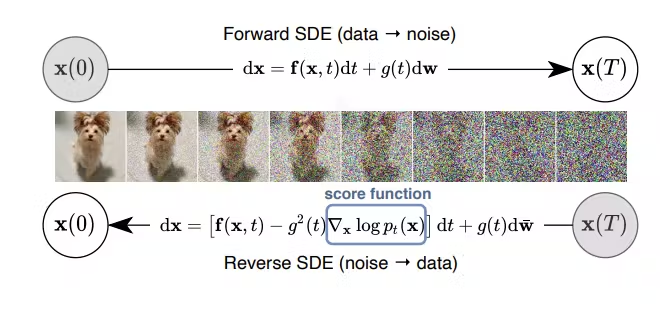
\includegraphics[width=0.9\textwidth]{figures/score_diffusion.png}
    \end{figure}
\end{itemize}
\end{column}
\begin{column}{0.48\textwidth}
\begin{itemize}\itemsep2pt
    \item An unnormalized density $\mu(x)$ where $D$ has density $\pi(x) \propto \mu(x)$ (e.g., 
    energy-based models, physics/chemistry)
    \begin{figure}
        \centering
        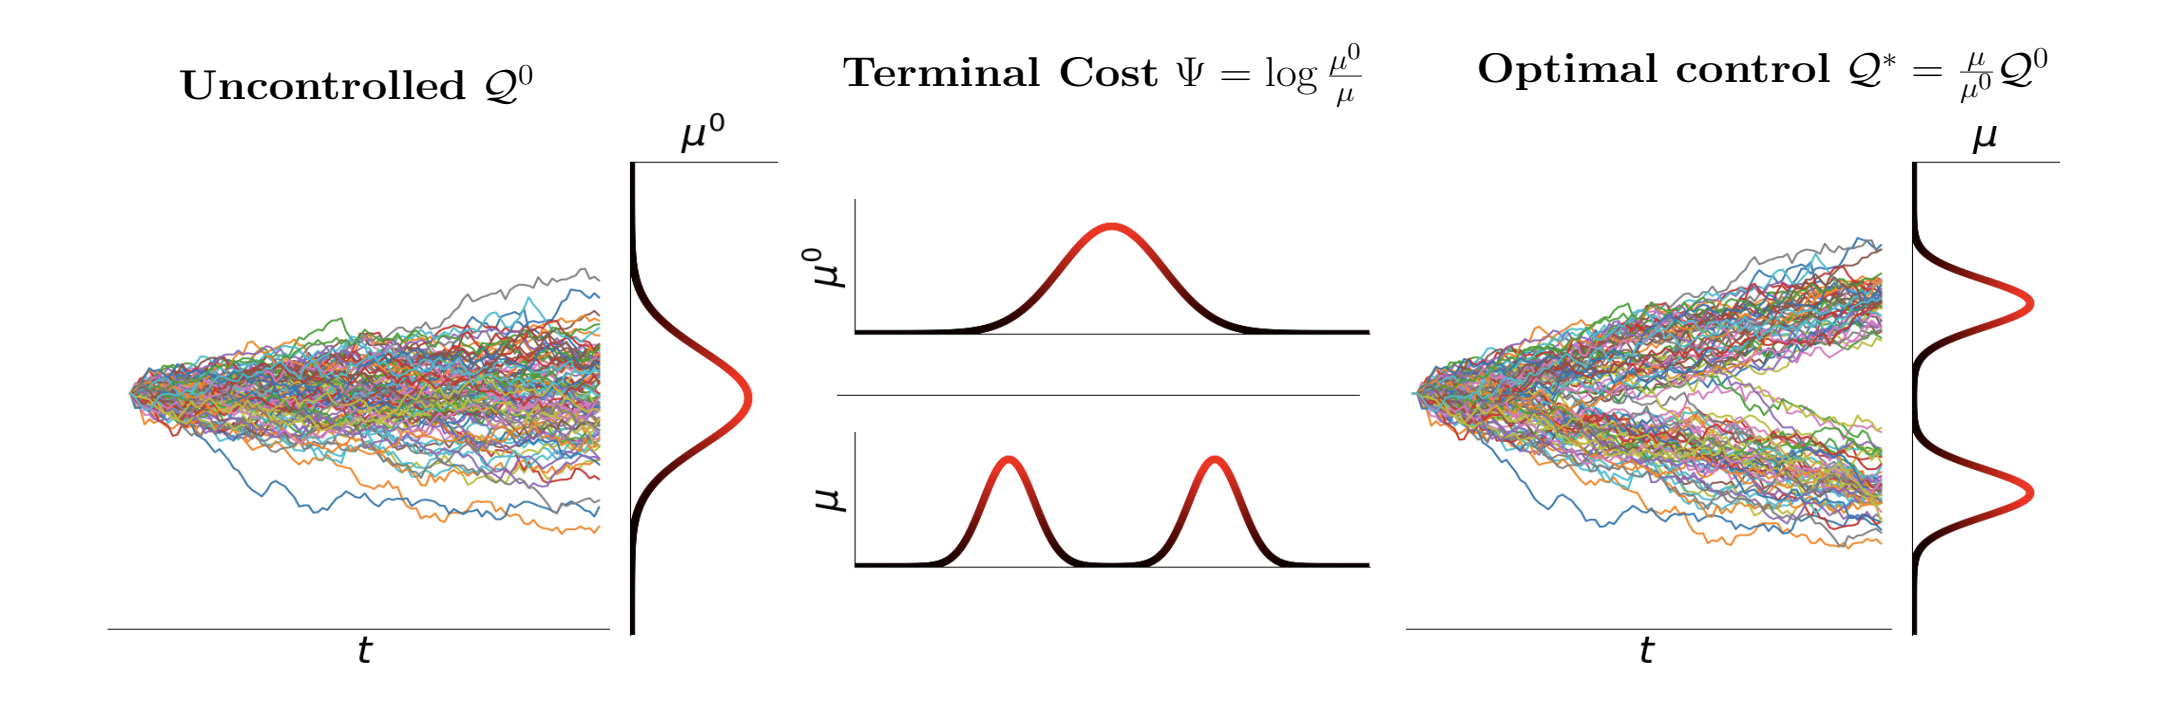
\includegraphics[width=0.9\textwidth]{figures/unconctrolled.png}
    \end{figure}
\end{itemize}
\end{column}
\end{columns}

\end{frame}

\begin{frame}[t]{Sampling from Unnormalized Densities}
\footnotesize
\textbf{Goal.} Sample from a $D$-dimensional target with unnormalized density $\mu(x)$ where $\mathbb R^D \to \mathbb R^+$.
\[
\pi(x)=\frac{\mu(x)}{Z},\qquad Z=\int_{\mathbb R^D}\mu(x)\,dx\ \text{(unknown)}.
\]
We assume we can evaluate $\mu(x)$, but we have no samples from $\pi$ and do not know $Z$.

\vspace{0.1cm}

\medskip
\textbf{Context.} We seek a \emph{sampler} (similar to MCMC/VI) that produces calibrated samples and, ideally, estimates of $\log Z$, \emph{without} any dataset from $\pi$.

\vspace{0.3cm}


\textbf{Chemistry (small-molecule conformers).} Different 3D conformations have a formation energy from force-field terms (bonds, angles, dihedrals, nonbonded); lower energy $\Rightarrow$ higher Boltzmann probability. A well-calibrated sampler is needed to draw conformers in proportion to these probabilities, which is important in binding-pose ranking/free-energy estimation, Boltzmann-weighted property prediction (e.g., NMR shifts), and generating diverse realistic 3D conformers for screening.
\end{frame}

\begin{frame}[t]{Diffusion Generative Flow Samplers}
\footnotesize
\textbf{Idea.} We will \emph{reframe sampling} from an unnormalized target $\pi(x)\propto \mu(x)$ as a \emph{stochastic optimal control (SOC)} problem: learn a control that steers a simple reference diffusion so its \emph{terminal marginal} matches $\pi$.

\medskip
\textbf{Why this helps.}
\begin{itemize}\itemsep2pt
  \item Gives a \emph{path-space} training objective/metric: a KL on trajectories $\mathrm{KL}(Q\,\|\,P)$ where $P$ is the reference paths reweighted by $\mu(x_T)$.
  \item The \emph{partition function $Z$ cancels} inside this objective, so we can train using only $\mu$ (and optionally $\nabla\log\mu$).
  \item Lets us optimize \emph{without samples from $\pi$} and still measure closeness to the true normalized endpoint.
\end{itemize}

\medskip
\textbf{Caveat (sets up DGFS).} This path-KL places supervision \emph{only at the terminal time} $\Rightarrow$ poor \emph{credit assignment} and high-variance gradients.

\medskip
\textbf{DGFS fix (preview).} Inject \emph{intermediate} learning signals via a GFlowNet-inspired \emph{learned flow} and \emph{subtrajectory balance}, enabling partial-trajectory training and more stable learning.
\end{frame}

\subsection{Stochastic Optimal Control}

% --- Slide 1 ---
\begin{frame}[t]{Steps 1--2: Forward \& Reference in \textit{discrete time}}
\footnotesize
\textbf{Controlled forward transition (learned drift).}
\[
P_F(x_{n+1}\mid x_n)\;=\;\mathcal N\!\big(x_{n+1};\;x_n + h\,f(x_n,n),\;h\sigma^2 I\big)
\]
\textbf{Controlled path law.}
\[
Q(x_{0:N})\;=\;p^{\text{ref}}_0(x_0)\;\prod_{n=0}^{N-1} P_F(x_{n+1}\mid x_n)
\]

\medskip
\textbf{Uncontrolled (reference) transition (zero drift).}
\[
P_F^{\text{ref}}(x_{n+1}\mid x_n)\;=\;\mathcal N\!\big(x_{n+1};\;x_n,\;h\sigma^2 I\big)
\]
\textbf{Reference path law and marginals.}
\[
Q^{\text{ref}}(x_{0:N})\;=\;p^{\text{ref}}_0(x_0)\;\prod_{n=0}^{N-1} P_F^{\text{ref}}(x_{n+1}\mid x_n),
\qquad p^{\text{ref}}_n(x)\;\text{is closed form.}
\]

\medskip
\textbf{Goal.} Learn $f$ so that the terminal marginal $Q(x_N)$ matches $\pi(x)=\mu(x)/Z$ (no data, $Z$ unknown).
\end{frame}

% --- Slide 2 ---
\begin{frame}[t]{Step 3: Path target \& KL $\Rightarrow$ SOC objective}
\scriptsize
% \textbf{Elementary identity: P(A,B) = P(A$\mid$B) P(B)}
% \[
% P(x_{0:N}) = P(x_{0:N-1} | x_N) P(x_N).
% \]

% \textbf{Reference bridge decomposition.}
% \[
% Q^{\text{ref}}(x_{0:N}) \;=\; Q^{\text{ref}}(x_{0:N-1}\mid x_N)\; p_N^{\text{ref}}(x_N),
% \qquad p_N^{\text{ref}}(x_N)=\!\int Q^{\text{ref}}(x_{0:N})\,dx_{0:N-1}.
% \]

\textbf{Target path measure via terminal reweighting.}
\[
P(x_{0:N}) \;\propto\; Q^{\text{ref}}(x_{0:N})\,\frac{\mu(x_N)}{p^{\text{ref}}_N(x_N)}
\qquad\Longrightarrow\qquad P(x_N)\propto\mu(x_N).
\]

\textbf{KL decomposition.}
\[
\mathrm{KL}(Q\|P)
=\mathbb E_{Q}\!\left[\log\frac{Q}{Q^{\text{ref}}}\right]
+\mathbb E_{Q}\!\left[\log\frac{p^{\text{ref}}_N(x_N)}{\pi(x_N)}\right].
\]
\medskip
\textbf{Running control cost (Gaussian mean-shift) Girsanov theorem.}
\[
\mathbb E_{Q}\!\left[\log\frac{Q}{Q^{\text{ref}}}\right]
=\mathbb E_Q \sum_{n=0}^{N-1}\frac{h}{2\sigma^2}\,\|f(x_n,n)\|^2.
\]

\textbf{Terminal potential from the target Girsanov theorem.}
\[
\mathbb E_{Q}\!\left[\log\frac{p^{\text{ref}}_N(x_N)}{\pi(x_N)}\right]
=\mathbb E_Q\!\big[\log p^{\text{ref}}_N(x_N)-\log \mu(x_N)\big]\;+\;\log Z.
\]

\end{frame}

\begin{frame}[t]{SOC objective}
\footnotesize
\medskip
\textbf{SOC objective (discrete-time).}
\[
\boxed{\ \min_{f}\ \mathbb E_Q\!\Big[\sum_{n=0}^{N-1}\tfrac{h}{2\sigma^2}\|f(x_n,n)\|^2\;+\;\log p^{\text{ref}}_N(x_N)-\log \mu(x_N)\Big]\ }
\]

we will be using this discrete-time objective as our loss function to optimize the drift $f$. Thus we can model the drift with a neural network $f_\theta$ and optimize the parameters $\theta$ backpropagating through time (BPTT) while avoiding to use the stochastic-adjoint method necessary for a neural SDE.
\end{frame}

%!Diffusion Denoising Score Matching slides removed for brevity 
% \begin{frame}[t]{Diffusion Process}
% \scriptsize

% \textbf{Idea.} Let the target “diffuse to Gaussian” via a reference process (VP/VE SDE). The \emph{reverse-time} dynamics can, in principle, generate target samples if we know the \emph{score} $\nabla_x \log p_t(x)$:
% \[
% \underbrace{dx_t=\sigma\,dW_t}_{\text{forward/noising}}
% \quad\Longleftrightarrow\quad
% \underbrace{dx_t=\big[f_{\text{ref}}(x,t)-\sigma^2\nabla_x \log p_t(x)\big]dt+\sigma\,d\bar W_t}_{\text{reverse/generative}}.
% \]

% \textbf{What is score matching?} 
% Learn a network $s_\theta(x,t)\approx \nabla_x\log p_t(x)$ by regressing on \emph{noised data}:
% \[
% \min_\theta\ \mathbb E_{t}\,\mathbb E_{x_0\sim p_{\text{data}}}\,\mathbb E_{\varepsilon}\!
% \big\|s_\theta(x_t,t)-\nabla_x\log p_t(x_t)\big\|^2,
% \]
% which is equivalent to denoising a corrupted sample $x_t$ back toward $x_0$.

% \vspace{0.1cm}
% \begin{errorblock}{Why Denoising Score Matching is \emph{not} applicable here}
% \begin{itemize}\itemsep2pt
%   \item We have \emph{no dataset} from $\pi$, only the unnormalized $\mu(x)$ (and maybe $\nabla\log\mu$).

% \end{itemize}
% \end{errorblock}

% \end{frame}
% \begin{frame}[t]{Alternative to DSM: learn the vector field (control)}
% \scriptsize
% \textbf{Reverse SDE drift (generative side).}
% \[
% dx_t=\big[f_{\text{ref}}(x,t)-\sigma^2\,\nabla_x \log p_t(x)\big]\,dt+\sigma\,d\bar W_t.
% \]

% \textbf{DSM route (data world).} Learn the \emph{score} $s_\theta(x,t)\approx\nabla_x\log p_t(x)$ from noised \emph{data}, then plug it into the reverse drift.

% \textbf{Vector-field route (our setting).} Directly learn the \emph{control/drift} $u_\theta(x,t)$ instead of the score. The two are \emph{equivalent} via:
% \[
% u_\theta(x,t)\;=\;f_{\text{ref}}(x,t)\;-\;\sigma^2\,s_\theta(x,t)
% \quad\Longleftrightarrow\quad
% s_\theta(x,t)\;=\;\tfrac{f_{\text{ref}}(x,t)-u_\theta(x,t)}{\sigma^2}.
% \]

% \textbf{Why do this here?}
% \begin{itemize}\itemsep2pt
%   \item We have no dataset from $\pi$, so DSM can’t form expectations over $p_t$; scores $\nabla\log p_t$ are unavailable.
%   \item Instead, treat $u_\theta$ as a \emph{control} and \emph{learn it} by minimizing a $Z$-free \textit{path-space} KL that uses only the given $\mu(\cdot)$.
%   \item This sets up diffusion samplers à la PIS/DDS and enables DGFS’s improvements (intermediate, subtrajectory credit).
% \end{itemize}

% \textbf{Notation tip.} Use $u_\theta$ (or $f$) for the vector field to avoid clashing with $\mu(\cdot)$, which denotes the unnormalized density.
% \end{frame}



%------------------------------------------------
\section{Diffusion Generative Flow Samplers}

\subsection{Motivation: Credit Assignment in Path Space}

\begin{frame}[t]{Credit Assignment Problem in Path Space}
\footnotesize
\begin{errorblock}{Current Loss Function}
\[
\min_{f}\ \mathbb E_Q\!\Big[\sum_{n=0}^{N-1}\tfrac{h}{2\sigma^2}\|f(x_n,n)\|^2\;+\;\log p^{\text{ref}}_N(x_N)-\log \mu(x_N)\Big]
\]
\end{errorblock}

\textbf{Explanation.} Since we are guiding our trajectory using the terminal marginal distribution $p_N^{\text{ref}}$ and $\mu(x)$, the only signal we have is at the end. Thus, when we do the chain rule for backpropagation through time, it is very hard to know which decision at which time step got the right or wrong action (credit assignment problem).

%running cost + terminal potential show optimal control base cost fucntion
\end{frame}

\begin{frame}{GFlowNet's perspective on DGFS}
\footnotesize

\textbf{Recap of GFlowNets.} GFlowNets learn to sample from unnormalized distributions by modeling flows on a DAG.

\begin{itemize}\itemsep2pt
  \item \textbf{DAG Structure:} Define a DAG $G = (S, A)$ with states $S$ and directed edges $s \to s' \in A$.
  \item \textbf{Trajectories:} Complete trajectories $\tau = s_0 \to s_1 \to \dots \to s_T$ from start to terminal states.
  \item \textbf{Forward Policy:} $P_F(s' | s)$, the probability of transitioning from $s$ to $s'$.
  \item \textbf{Terminal Marginal:} $P_T(x) = \sum_{\tau \text{ ending at } x} P_F(\tau)$, the marginal over terminating states.
  \item \textbf{Goal:} Learn $P_F$ such that $P_T(x) \propto R(x)$, where $R(x)$ is the unnormalized reward/density, and $Z = \sum_x R(x)$.
\end{itemize}

\end{frame}

\begin{frame}[t]{SOC as a GFlowNet}
\footnotesize

\textbf{Comparison Table: GFlowNet vs. SOC Framework}

\begin{table}[h]
\centering
\footnotesize
\begin{tabular}{@{}lcccc@{}}
\toprule
\textbf{Concept} & \textbf{GFlowNet} & \textbf{SOC} \\
\midrule
\textbf{Forward Process} & Trajectory sampling on DAG & Controlled diffusion path \\
\textbf{Forward Transition Probability} & $P_F(s' | s)$ & $P_F(x_{n+1} | x_n) = \mathcal{N}(x_{n+1}; x_n + h f(x_n), h\sigma^2 I)$ \\
\textbf{Reward Function} & $R(x)$ (unnormalized) & $\mu(x)$ (unnormalized density) \\
\textbf{Terminal Marginal Distribution} & $P_T(x) \propto R(x)$ & $Q(x_N) \propto \mu(x_N)$ \\
\textbf{Flow State} & Flow $F(s)$ at states & Learned flow $F_n(x)$ \\
\bottomrule
\end{tabular}
\end{table}

\textbf{Insight.} Since SOC can be viewed as a GFlowNet, we can apply GFlowNet tools (e.g., detailed balance loss, subtrajectory balance) to solve the credit assignment problem in diffusion sampling.

\end{frame}

\begin{frame}[t]{Insight in solving credit assignment problem}
\footnotesize

\textbf{What if we could know or approximate the target distribution at any step $n$?}

\[
P(x_0, \dots, x_N) := Q^{\text{ref}}(x_0, \dots, x_N) \frac{\pi(x_N)}{p^{\text{ref}}_N(x_N)}.
\]

Using the reference bridge decomposition:
\[
Q^{\text{ref}}(x_{0:N}) = Q^{\text{ref}}(x_{0:N-1} | x_N) \, p_N^{\text{ref}}(x_N),
\qquad p_N^{\text{ref}}(x_N) = \int Q^{\text{ref}}(x_{0:N}) \, dx_{0:N-1}.
\]

\[
P(x_{0:N}) = \pi(x_N) \prod_{n=0}^{N-1} P_B(x_n | x_{n+1}),
\]

Unfortunately, although we know the form of $P_B(\cdot|\cdot)$, for general target distribution there is generally no known analytical expression for it. As a result, we propose to use a deep neural network $F_n(\cdot; \theta)$ with parameter $\theta$ as a “helper” to approximate the unnormalized density of the $n$-th step target $p_n(\cdot)$.
\end{frame}

\begin{frame}[t]{Training the Flow Network: Naive Approach}
\footnotesize

\textbf{Naive Way to Train $F_n(\cdot; \theta)$.} One simple method is to fit $F_n$ to a Monte Carlo (MC) quadrature estimate of the integral in Equation 11 (which approximates the unnormalized density at step $n$).

\textbf{Why Not?} Every training step requires a computationally expensive quadrature calculation (e.g., sampling many trajectories to estimate the integral). This makes the algorithm extremely inefficient, as MC quadrature is slow and scales poorly with dimensionality.

\textbf{Decision.} Instead of direct quadrature per step, amortize the computation by turning it into an optimization problem that learns $F_n$ end-to-end.

\end{frame}

\begin{frame}[t]{Amortized Training: The Subtrajectory Constraint}
\footnotesize

\textbf{Proposed Amortized Approach.} Train $F_n(\cdot; \theta)$ to satisfy the following constraint for all partial trajectories $x_{n:N}$:
\[
F_n(x_n; \theta) \prod_{l=n}^{N-1} P_F(x_{l+1} | x_l; \theta) = \mu(x_N) \prod_{l=n}^{N-1} P_B(x_l | x_{l+1}).
\]

\textbf{Details.}
\begin{itemize}\itemsep2pt
  \item $P_F$ (forward policy) and $F_n$ are parameterized by deep neural networks.
  \item Once this constraint holds, $F_n(x_n; \theta)$ equals the integral in Equation 11, amortizing the integration into the learning of $\theta$.
  \item We use only $\mu(\cdot)$ (no $Z$), so the unknown normalization is absorbed into $F_n$.
\end{itemize}

\textbf{Decision.} This avoids per-step quadrature by enforcing a global constraint on partial trajectories, making training efficient and scalable.

\end{frame}

\begin{frame}[t]{Training Objective and Implementation}
\footnotesize

\textbf{Training Objective.} Regress the left-hand side (LHS) of the constraint to the right-hand side (RHS). For stability, perform this in log space:
\[
\min_\theta \left| \log(\text{LHS}) - \log(\text{RHS}) \right|.
\]

\textbf{Details.}
\begin{itemize}\itemsep2pt
  \item This is a regression loss that minimizes the difference between the learned flow products and the target products involving $\mu$.
  \item Log space prevents numerical issues from large or small values.
\end{itemize}

\textbf{Shared Parameters.} The flow function at different steps shares the same parameters; achieved by adding a step embedding input to the network $F(\cdot, n; \theta)$.

\textbf{Decision.} Sharing parameters reduces model complexity and ensures consistency across time steps, while embeddings allow step-specific behavior.

\end{frame}

\begin{frame}[t]{Derived Subtrajectory Balance (SubTB)}
\footnotesize

\textbf{Deriving SubTB.} Comparing the constraint for $n$ and $n+1$ gives a formula independent of $\mu$:
\[
F_n(x_n; \theta) P_F(x_{n+1} | x_n; \theta) = F_{n+1}(x_{n+1}; \theta) P_B(x_n | x_{n+1}).
\]

\textbf{Details.}
\begin{itemize}\itemsep2pt
  \item This is the Subtrajectory Balance (SubTB) constraint, a generalization of detailed balance for partial trajectories.
  \item It provides intermediate learning signals without needing $\mu$ directly, improving credit assignment.
\end{itemize}

\textbf{Overall Decision.} The method learns two neural networks: the flow $F(\cdot, n; \theta)$ and the forward policy $P_F$. This setup enables efficient, stable training with intermediate supervision.

\end{frame}

\begin{frame}[t]{DGFS algorithm}

    \begin{figure}
        \centering
        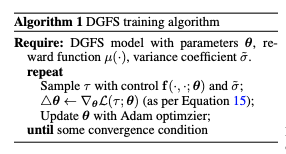
\includegraphics[width=0.9\textwidth]{figures/algo.png}
    \end{figure}

\end{frame}

% \begin{frame}[t]{Intermediate Learning Signals}

% \footnotesize
% \textbf{Key Idea.} Instead of waiting for the final signal, DGFS uses \emph{subtrajectory balance (SubTB)} to provide intermediate learning signals by optimizing over partial trajectories.

% \begin{block}{Detailed Balance (DB) Loss in GFlowNets}
% \[
% \ell_{\text{DB}}(s, s'; \theta) = \left( \log \frac{F(s; \theta) P_F(s'|s; \theta)}{F(s'; \theta) P_B(s|s'; \theta)} \right)^2
% \]
% According to the theory of GFlowNets (Bengio et al., 2023), if the DB loss reaches 0 for any transition pair, then the forward policy samples correctly from the target distribution defined by R(·).

% \end{block}

% \begin{itemize}
%     \item s and s' are two states in the trajectory (e.g., $x_n$ and $x_{n+1}$).
%     \item F(s; $\theta$) is the learned flow function at state s, $P_F(s'|s; \theta)$ is the forward transition probability from s to s', and $P_B(s|s'; \theta)$ is the backward transition probability from s' to s.
% \end{itemize}

% \end{frame}


%------------------------------------------------
\section{Results and Limitations}

\subsection{Results}


%------------------------------------------------
\section{Conclusion}

\subsection{Key Insights}
% Add content: Summarize DGFS's impact and paper's contributions.

\subsection{Future Directions and Usage since its release}
% Add content: Discuss limitations, extensions, and personal thoughts.

\begin{frame}{Conclusion}

\end{frame}


\end{document}